% Drawing 154/08-10 -- folder 154, batch 08, archive page 155 (PDF page 156).
% Transcription: page de dessins au crayon et à l'encre brune et verte, dans les conventions de la page 154 : en haut, un fuseau brun bordé de droites qui se croisent en losanges, et au-dessous un fuseau au crayon ; au milieu, des croisements de droites, un fuseau au crayon parcouru d'un zigzag brun entre ses deux rives (sept sommets) ; une courbe brune qui s'abaisse en tirets pour passer par un sommet ; une bosse brune et verte sur une droite en tirets ; en bas, quatre dessins de bandes : une droite verte bordée de deux courbes brunes qui s'écartent en bosses pour passer par des sommets (un en haut, un en bas ; puis un en haut, deux en bas), et un petit fuseau avec deux flèches opposées
% Kind: page of spindles and crossings in the conventions of p. 154 (pencil, brown and green ink). Method 2 (schematic redraw from the facsimile). Status: partial.
% Notes: Page of drawings in pencil and brown and green ink over a printed notice (not reproduced), read from the page view: at the top a brown spindle bordered by lines crossing in lozenges, and below it a pencil spindle; in the middle crossings of lines, a pencil spindle run through by a brown zigzag between its two banks (seven vertices marked), a bump of a line over a crossing; at the bottom, brown spindles round a green line whose banks bulge over the crossings (the last of them carries the legends of 08-11). Many pencil lines are left out. Still differs from the facsimile: Page of drawings in pencil and brown and green ink over a printed notice (not reproduced), read from the page view: at the top a brown spindle bordered by lines crossing in lozenges, and below it a pencil spindle; in the middle crossings of lines, a pencil spindle run through by a brown zigzag between its two banks (seven vertices marked), a bump of a line over a crossing; at the bottom, brown spindles round a green line whose banks bulge over the crossings (the last of them carries the legends of 08-11). Many pencil lines are left out.
% Coordinates: 1 unit = 1 mm = 1/100 of the crop width (bbox in page fractions: [0.121, 0.073, 0.937, 0.521]).
% Redrawn by Claude (claude-opus-5-5), issue #73, 2026-11-07; not checked by a human; not compiled (no TeX in the session).
% Revised by Claude (claude-opus-5-5) 2026-11-09 (issue #128) after Michel's check: vertices snapped to exact intersections (drawn points on their lines, meeting ends on the stroke they meet, near-concurrent lines through one computed point, curve ends on their rim); labels at \small as in folder 80 batch 3. Status: partial.
% Rights: reproduces part of the work -- behind RENDER_TRANSCRIPTS, never published by itself.
\documentclass[tikz,border=3pt]{standalone}
\usepackage{amsmath,amssymb}
\usetikzlibrary{patterns,arrows.meta}
\tikzset{Or/.style={orange!90!black}, Ye/.style={yellow!80!orange}, Lg/.style={green!60!black!70}, Dg/.style={green!45!black}, Br/.style={brown!80!black}, Rd/.style={red!85!black}, Bl/.style={blue!70!black}, Gy/.style={black!40}, pencil/.style={black!45}, struck/.style={black!35}, mark/.style={circle,draw,inner sep=1.3pt}, pt/.style={circle,fill,inner sep=0.9pt}, opt/.style={circle,draw,fill=white,inner sep=1.1pt}}
\begin{document}
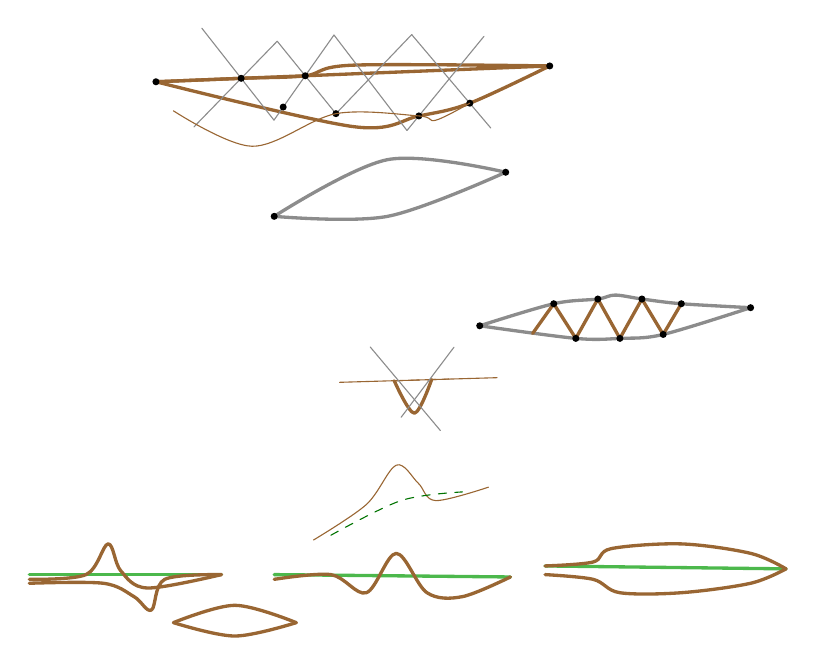
\begin{tikzpicture}[x=1mm,y=1mm,line cap=round,line join=round,font=\scriptsize]
\draw[Br,very thick] plot[smooth, tension=0.55] coordinates {(18.88,-5.71) (29.7,-5.27) (37.84,-4.95) (43.9,-3.6) (68.89,-3.7)};
\draw[Br,very thick] plot[smooth, tension=0.55] coordinates {(18.88,-5.71) (43.9,-11.4) (52.27,-10.05) (58.74,-8.43) (68.89,-3.7)};
\draw[Br,very thick] (18.88,-5.71) -- (68.89,-3.7);
\draw[pencil] (24.71,1.09) -- (33.87,-10.58);
\draw[pencil] (34.28,-0.56) -- (23.71,-11.44);
\draw[pencil] (34.28,-0.56) -- (41.74,-9.76);
\draw[pencil] (41.49,0.23) -- (33.87,-10.58);
\draw[pencil] (41.49,0.23) -- (50.76,-11.9);
\draw[pencil] (51.36,0.28) -- (41.74,-9.76);
\draw[pencil] (51.36,0.28) -- (61.4,-11.58);
\draw[pencil] (60.53,0.05) -- (50.76,-11.9);
\node[pt] at (18.88,-5.71) {};
\node[pt] at (29.7,-5.27) {};
\node[pt] at (37.84,-4.95) {};
\node[pt] at (35.04,-8.92) {};
\node[pt] at (41.74,-9.76) {};
\node[pt] at (52.27,-10.05) {};
\node[pt] at (58.74,-8.43) {};
\node[pt] at (68.89,-3.7) {};
\draw[Br] plot[smooth, tension=0.55] coordinates {(21.1,-9.4) (31.1,-13.9) (41.74,-9.76) (52.27,-10.05) (54.4,-10.6) (58.74,-8.43)};
\draw[pencil,very thick] plot[smooth, tension=0.55] coordinates {(33.9,-22.8) (48.3,-15.6) (63.3,-17.2)};
\draw[pencil,very thick] plot[smooth, tension=0.55] coordinates {(33.9,-22.8) (48.3,-22.8) (63.3,-17.2)};
\node[pt] at (33.9,-22.8) {};
\node[pt] at (63.3,-17.2) {};
\draw[pencil,very thick] plot[smooth, tension=0.55] coordinates {(60,-36.7) (69.4,-33.9) (75,-33.3) (77.2,-32.8) (80.6,-33.3) (85.6,-33.9) (94.4,-34.4)};
\draw[pencil,very thick] plot[smooth, tension=0.55] coordinates {(60,-36.7) (72.2,-38.3) (77.8,-38.3) (83.3,-37.8) (94.4,-34.4)};
\draw[Br,very thick] (66.72,-37.67) -- (69.4,-33.9) -- (72.2,-38.3) -- (75,-33.3) -- (77.8,-38.3) -- (80.6,-33.3) -- (83.3,-37.8) -- (85.6,-33.9);
\node[pt] at (60,-36.7) {};
\node[pt] at (94.4,-34.4) {};
\node[pt] at (69.4,-33.9) {};
\node[pt] at (75,-33.3) {};
\node[pt] at (80.6,-33.3) {};
\node[pt] at (85.6,-33.9) {};
\node[pt] at (72.2,-38.3) {};
\node[pt] at (77.8,-38.3) {};
\node[pt] at (83.3,-37.8) {};
\draw[Br] (42.2,-43.88) -- (62.2,-43.29);
\draw[Br,very thick] plot[smooth, tension=0.55] coordinates {(49.15,-43.69) (51.7,-47.8) (53.89,-43.53)};
\draw[Br,dashed] (49.15,-43.69) -- (56.11,-43.46);
\draw[pencil] (46.1,-39.4) -- (55,-50);
\draw[pencil] (56.73,-39.42) -- (50.02,-48.32);
\draw[Br] plot[smooth, tension=0.55] coordinates {(38.9,-63.9) (45.6,-59.4) (49.4,-54.4) (52.2,-56.7) (54.4,-58.9) (61.1,-57.2)};
\draw[Dg,dashed] plot[smooth, tension=0.55] coordinates {(41.1,-63.3) (50,-58.9) (57.8,-57.8)};
\draw[Lg,very thick] (2.8,-68.3) -- (27.2,-68.3);
\draw[Lg,very thick] (33.9,-68.3) -- (63.9,-68.6);
\draw[Lg,very thick] (68.3,-67.2) -- (98.9,-67.57);
\draw[Br,very thick] plot[smooth, tension=0.55] coordinates {(2.8,-68.9) (10,-68.3) (12.8,-64.4) (14.4,-67.8) (17.8,-70) (27.2,-68.3)};
\draw[Br,very thick] plot[smooth, tension=0.55] coordinates {(2.8,-69.4) (12.2,-69.4) (16.1,-71.1) (18.3,-72.8) (20,-68.9) (27.2,-68.3)};
\draw[Br,very thick] plot[smooth, tension=0.55] coordinates {(33.9,-68.9) (41.1,-68.3) (45.6,-70.6) (49.4,-65.6) (53.3,-70.6) (57.8,-71.1) (63.9,-68.6)};
\draw[Br,very thick] plot[smooth, tension=0.55] coordinates {(21.1,-74.4) (28.9,-72.2) (36.7,-74.4)};
\draw[Br,very thick] plot[smooth, tension=0.55] coordinates {(21.1,-74.4) (28.9,-76.1) (36.7,-74.4)};
\draw[Br,very thick] plot[smooth, tension=0.55] coordinates {(68.3,-67.2) (74.4,-66.7) (76.7,-65) (85.6,-64.4) (94.4,-65.6) (98.9,-67.57)};
\draw[Br,very thick] plot[smooth, tension=0.55] coordinates {(68.3,-68.3) (74.4,-68.9) (77.8,-70.6) (85.6,-70.6) (94.4,-69.4) (98.9,-67.57)};
\end{tikzpicture}
\end{document}
